\section{Theorie}
\label{sec:theorie}

    Im folgenden Abschnitt werden die theoretischen Grundlagen der Relaxation eines RC-Kreises erläutert.

\subsection{Relaxationsphänomene}

    Ein System zeigt Relaxationsverhalten,
    wenn es aus seinem Ausgangszustand gebracht wird und es nicht-oszillatorisch in den Ausgangszustand zurückkehrt.
    Die zeitliche Änderung der beobachteten Größe $A$ ist dabei proportional zu ihrer Abweichung vom Endzustand $A(\infty))$,
    welcher nur asymptotisch erreicht wird
    \begin{equation*}
        \frac{\symup{d}A}{\symup{d}t} = c(A(t) - A(\infty)) \ .
    \end{equation*}
    Integration liefert die Relaxationsgleichung der Größe $A$,
    wobei der Faktor $c < 0$ ist.
    Es gilt
    \begin{equation*}
        A(t) = A(\infty) + (A(0) - A(\infty)) \cdot \symup{e}^{ct} \ .
    \end{equation*}

\subsection{Auf- und Entladevorgang eines Kondensators}

    Als Beispiel für Relaxationsverhalten dient die Auf- und Entladung eines Kondensators.

    \begin{figure}
        \centering
        \includegraphics{content/img/Abb_1.pdf}
        \caption{Schaltung des Auf- und Entladevorgangs eines Kondensators.}
        \label{fig:schaltung_kondensatorEntAufladung}
    \end{figure}

    In Abbildung \ref{fig:schaltung_kondensatorEntAufladung} ist die Schaltung dargestellt,
    die zur Messung der Auf- und Entladung des Kondensators verwendet wird.\\
    Für den Entladevorgang wird der Schalter in der Schaltung in Position 1 gebracht.
    Auf dem Kondensators mit der Kapazität $C$ ist eine Ladungsmenge $Q$ gespeichert.
    Zwischen den Platten liegt eine Spannung $U_\text{C}$ an,
    die mithilfe von
    \begin{equation}
        U_\text{C} = \frac{Q}{C}
        \label{eqn:kondensatorspannung}
    \end{equation}
    berechnet werden kann.
    Für den Strom ergibt sich
    \begin{equation}
        I = \frac{U_\text{C}}{R} \ ,
        \label{eqn:strom_ohmgesetz}
    \end{equation}
    mit dem ohm'schen Widerstand $R$.
    Der zeitliche Verlauf der Ladung wird mithilfe der Differentialgleichung
    \begin{equation}
        \frac{\symup{d}Q}{\symup{d}t} = I(t) = - \frac{1}{RC} Q(t)
        \label{eqn:dgl_ladung}
    \end{equation}
    beschrieben,
    mit der Lösung
    \begin{equation}
        Q(t) = Q(0) \exp{\Bigl(- \frac{t}{RC}\Bigr)} \ ,
        \label{eqn:entladung}
    \end{equation}
    wobei der Kondensator nach unendlicher Zeit entladen ist,
    also $Q(\infty) = 0$. \\
    Für den Aufladevorgang wird der Schalter in der Schaltung in Position 2 gebracht.
    An dem Kondensator ist eine Spannung $U_0$ angebracht und es gelten die Randbedingungen
    \begin{align*}
        Q(0) &= 0 & Q(\infty) = C U_0 \ .
    \end{align*}
    Für den zeitlichen Verlauf der Ladung ergibt sich analog
    \begin{equation}
        Q(t) = C U_0 (1 - \exp{\Bigl(-\frac{t}{RC}\Bigr)}) \ .
        \label{eqn:aufladung}
    \end{equation}
    \\
    Die Zeitkonstante $RC$ gibt die Geschwindigkeit an,
    mit der das System in seinen Endzustand $Q(\infty)$ strebt.
    In der Zeit $\symup{\Delta}T = RC$ ändert sich die Ladung um $\frac{Q(t=RC)}{Q(0)}$.

\subsection{Relaxationsphänomene bei periodischer Auslenkung}

    Das Relaxationsverhalten eines RC-Kreises kann bei Anlegen einer Wechselspannung $U(t) = U_0 \cos(\omega t)$ als Beispiel für andere Gebiete der Physik darstellen.

    \clearpage
    \begin{figure}
        \centering
        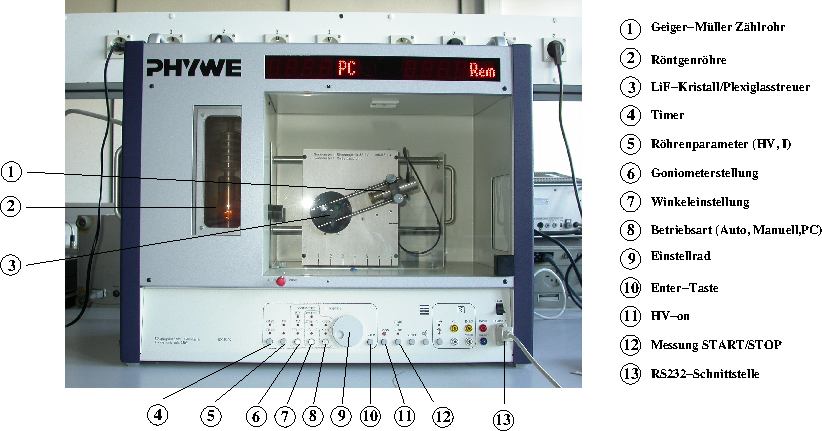
\includegraphics{content/img/Abb_2.pdf}
        \caption{Schaltung zur Beobachtung von Relaxationsverhalten bei periodischer Auslenkung.}
        \label{fig:schaltung_wechselspannung}
    \end{figure}

    Die Abbildung \ref{fig:schaltung_wechselspannung} zeigt die dafür verwendete Schaltung.
    Für hinreichend kleine Kreisfrequenz $\omega << \frac{1}{RC}$ gilt $U_\text{C}(t) = U(t)$,
    wobei bei steigender Frequenz eine Phasenverschiebung $\phi$ zwischen der Kondensatorspannung und der Generatorspannung $U_\text{G}(t)$ auftritt.
    Die Spannung $U(t)$ setzt sich nach der zweiten Kirchhoff'schen Regel aus der Spannung am Widerstand $U_\text{R}$ und der Spannung am Kondensator,
    für die
    \begin{equation}
        U_\text{C} = A(\omega) \cos{(\omega t + \phi(\omega))}
    \end{equation}
    gilt,
    zusammen.
    Die Spannung $U(t)$ ist für alle Zeiten $t$ gültig,
    sodass sich mit einigen Umformungen die Phasenverschiebung
    \begin{equation}
        \phi(\omega) = \arctan{(- \omega RC)}
        \label{eqn:phasenverschiebung}
    \end{equation}
    ergibt,
    wobei $\phi$ für kleine Frequenzen gegen Null geht und sich für hohe Frequenzen asymptotisch an $\frac{\symup{\pi}}{2}$ annähert.
    Für die Amplitude ergibt sich mithilfe von $\omega t + \symup{\phi} = \frac{\symup{\pi}}{2}$ die folgende Beziehung
    \begin{equation}
        A(\omega) = \frac{U_0}{\sqrt{1 + {\omega}^2 R^2 C^2}} \ .
        \label{eqn:amplitude}
    \end{equation}
    Für kleine Frequenzen $\omega \to 0$ geht $A(\omega)$ gegen $U_0$ und für hohe Frequenzen $\omega \to \infty$ geht $A(\omega)$ gegen Null.\\
    Ein RC-Kreis mit anliegender Wechselspannung kann auch als Tiefpass verwendet werden,
    da er Frequenzen,
    die klein gegen $\frac{1}{RC}$ sind,
    ungehindert durchlässt und Frequenzen mit $\omega >> \frac{1}{RC}$ herunterteilt.

\subsection{RC-Kreis als Integrator}

    Für hinreichend kleine Frequenzen $\omega >> \frac{1}{RC}$ gilt
    \begin{equation*}
        U_\text{C} \propto \int U(t) \symup{d}t \ .
    \end{equation*}
    Es ergibt sich für die Spannung $U(t)$ wieder der folgende Zusammenhang
    \begin{equation}
        U(t) = U_\text{R} + U_\text{C} \ ,
    \end{equation}
    wobei $U_\text{R} = RC \frac{\symup{d}U_\text{C}}{\symup{d}t}$ nach der Beziehung in Gleichung \eqref{eqn:dgl_ladung} verwendet wird.
    Mit $\lvert U_\text{C} \rvert \ll \lvert U_\text{R} \rvert$ und $\lvert U_\text{C} \rvert \ll \lvert U \rvert$ gilt für die Spannung am Kondensator
    \begin{equation}
        U_\text{C} = \frac{1}{RC} \int_0^1 U(t') \symup{d}t' \ .
        \label{eqn:integrator}
    \end{equation}
